\chapter{Mobile Application: English Mind}
\label{chap:mobile-application-english-mind}

English Mind is a mobile application available on Android \cite{cite:english_mind_play_store} and iOS \cite{cite:english_mind_app_store} platforms that focuses on learning English vocabulary. To achieve high efficiency in learning new English vocabulary, the application combines three main teaching methods on which it is based \cite{cite:english_mind_website}:

\begin{itemize}
    \item Frequency list of English vocabulary
    \item Active recall utilizing flashcards
    \item Spaced repetition system
\end{itemize}

These methods create a structured and efficient approach to mastering vocabulary with minimal effort, setting the app apart from its competitors in the field of vocabulary learning apps.

\section{Frequency List}

A frequency list ranks words according to their occurrence in common texts and speech. This approach is particularly valuable in vocabulary teaching for foreign language learners, as learning high-frequency words first enables students to comprehend more of their target language earlier in their studies.

Research by Nation \cite{cite:nation2006_how_large_vocabulary_is_needed} demonstrates the effectiveness of this approach. Mastering the 1,000 most frequent word families enables understanding of 78-81\% of written text, while 8,000-9,000 word families are required for 98\% comprehension. This data underscores the importance of prioritizing high-frequency vocabulary in language acquisition.\newpage

The frequency list implementation in English Mind allows users to browse words and assign them one of three states: UNSEEN (default), KNOWN, and LEARNING. Users can modify these states as shown in Figure \ref{fig:em-frequency-list}. Words marked as "LEARNING" are practiced using flashcards and scheduled for review through spaced repetition.

\begin{figure}[!h]
    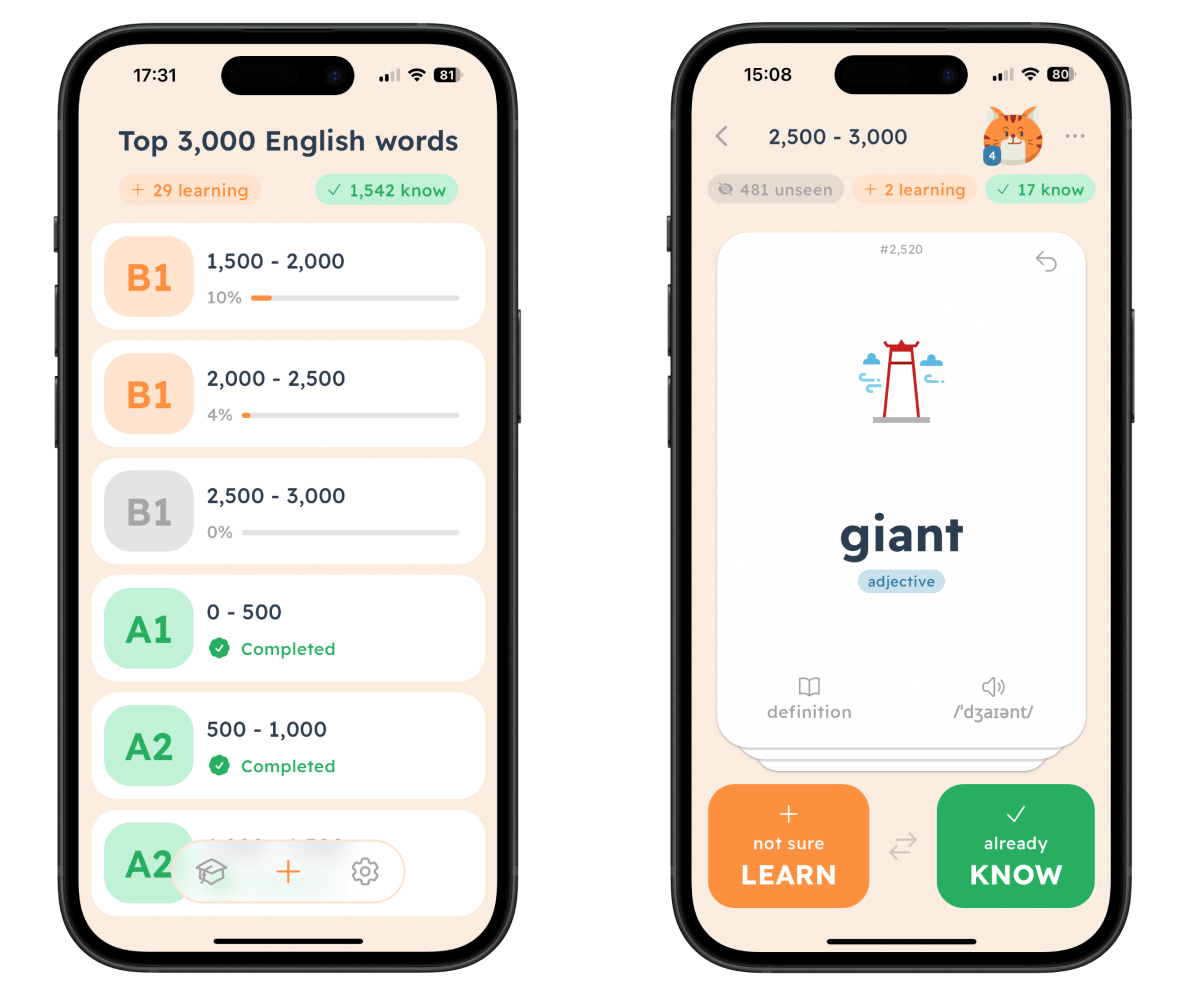
\includegraphics[width=0.8\textwidth]{src/figures/em-frequency-list.png}
    \caption{English Mind - Frequency List}
    \label{fig:em-frequency-list}
\end{figure}

\section{Active Recall and Flashcards}
\label{sec:em-active-recall}

Active recall is a learning method where students attempt to retrieve information without reference to the source material, contrasting with passive review where information is simply reread. Research from Washington University \cite{cite:rhkj2006_longterm_retention} demonstrates active recall's superiority for long-term retention: in a study of 120 students, active recall consistently outperformed passive review across various time intervals (5 minutes, 2 days, and 1 week), as shown in Figure \ref{fig:active-recall-passive-review-results}.

\begin{figure}[!h]
    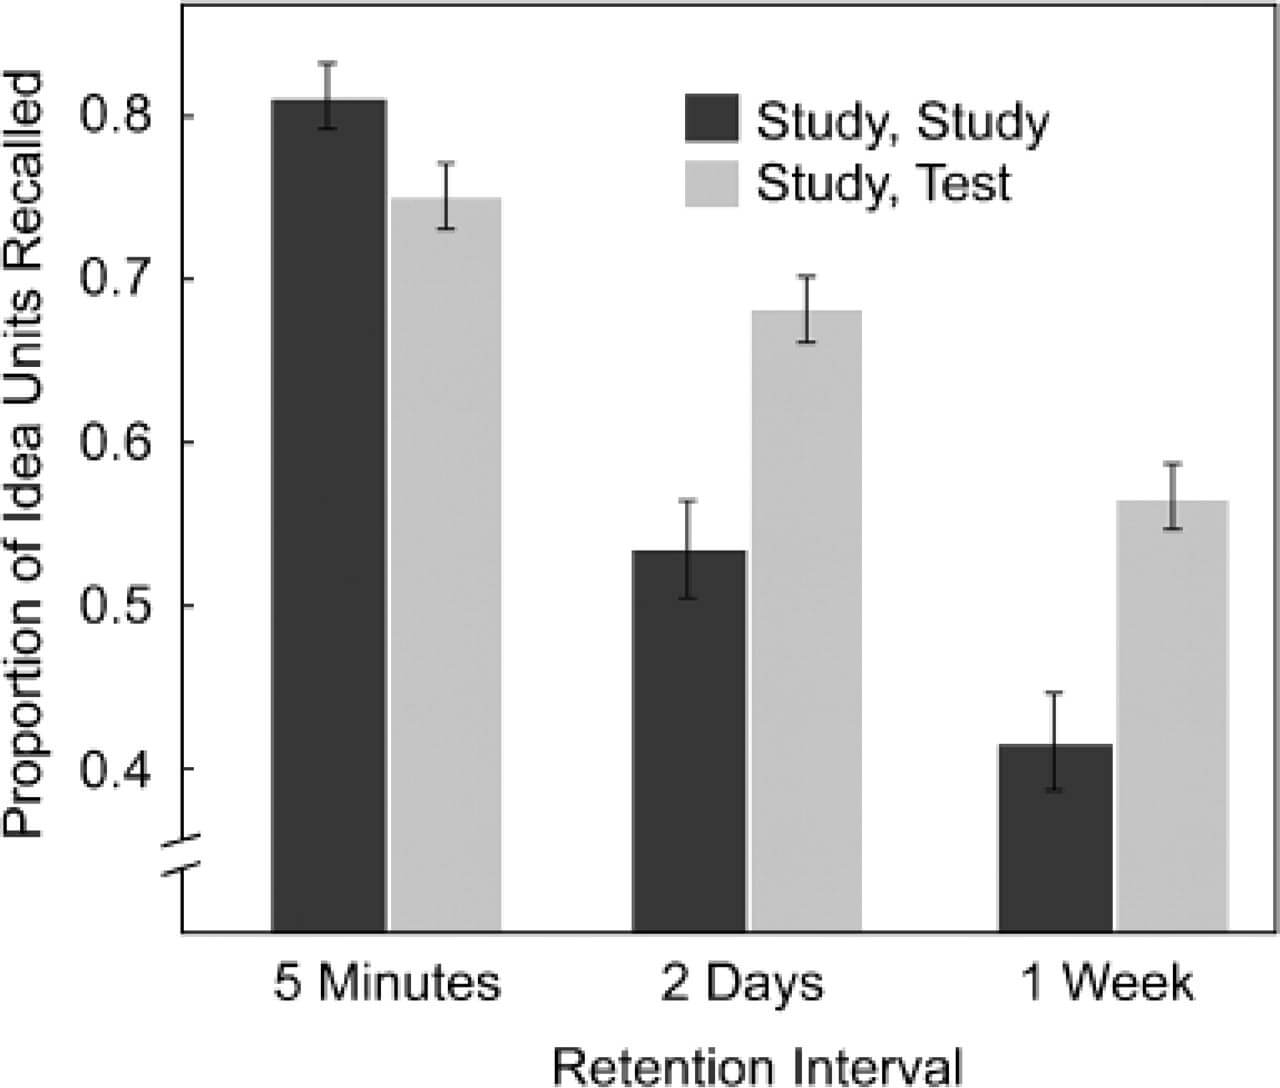
\includegraphics[width=0.7\textwidth]{src/figures/active-recall-passive-review-results.jpeg}
    \caption{Comparison of retention rates between active recall and passive review methods across different time intervals \cite{cite:rhkj2006_longterm_retention}}
    \label{fig:active-recall-passive-review-results}
\end{figure}

Flashcards represent a practical implementation of active recall, where information is split between two sides of a card, forcing active retrieval before verification.

English Mind implements flashcard-based active recall by presenting vocabulary words on the front and comprehensive word information (definition, usage examples, pronunciation, and native language translation) on the reverse, as shown in Figure \ref{fig:em-flashcards}. Users must attempt to recall the word's meaning before revealing the reverse side.

\begin{figure}[!h]
    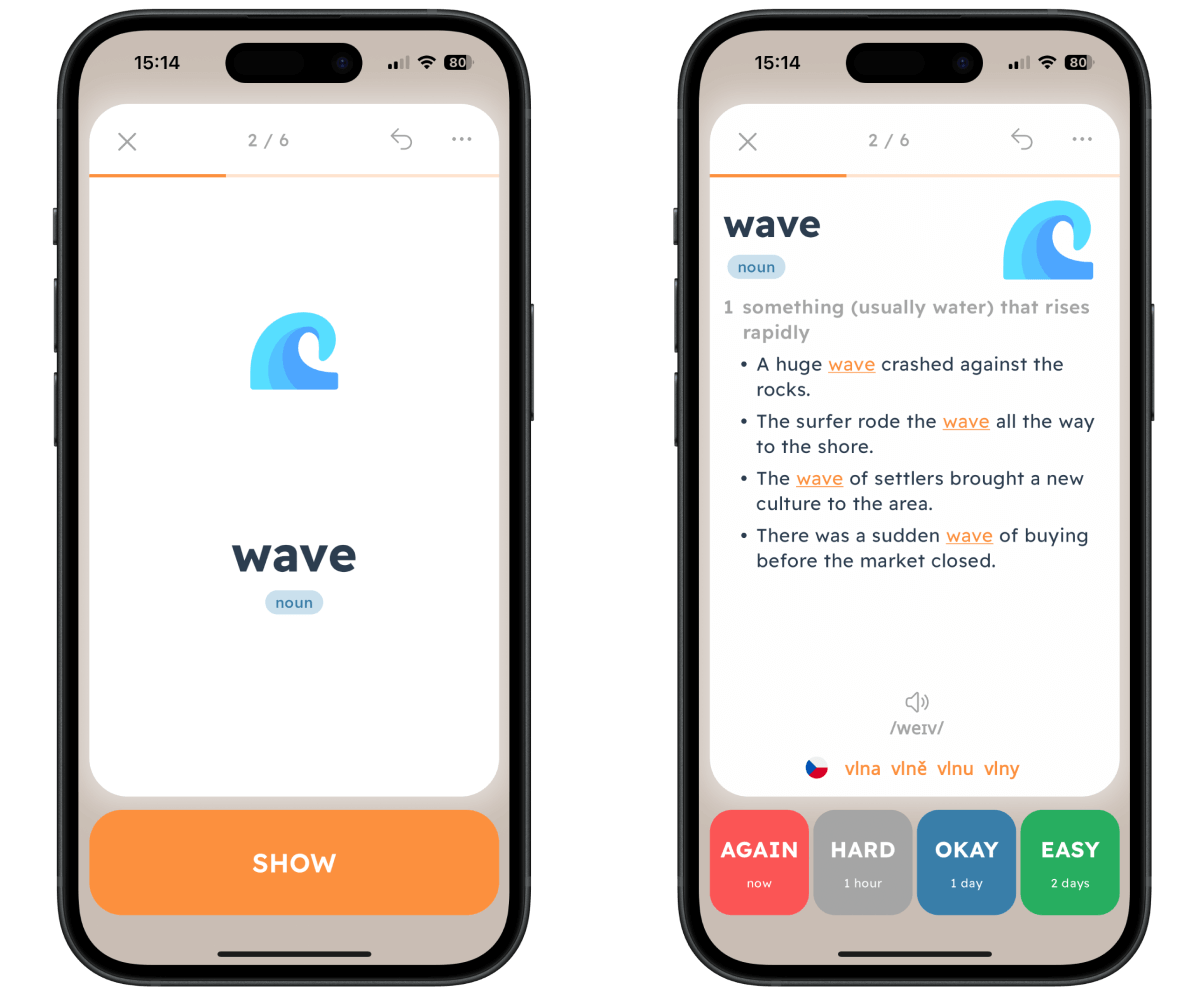
\includegraphics[width=0.9\textwidth]{src/figures/em-flashcards.png}
    \caption{English Mind - Active Recall Utilizing Flashcards}
    \label{fig:em-flashcards}
\end{figure}

\section{Spaced Repetition System (SRS)}

Spaced Repetition System (SRS) optimizes learning by adjusting intervals between review sessions based on recall performance. This method builds on Ebbinghaus's forgetting curve theory \cite{cite:ebbinghaus2013_memory_contribution_to_experimantal_psychology}, which demonstrates that information retention improves when review occurs just before predicted forgetting. Research shows that SRS increases learning efficiency by optimizing review timing and reducing unnecessary repetition \cite{cite:kang2016_spaced_repetiton_promotes_efficient_learning}.

The application implements SRS through a four-button feedback system (AGAIN, HARD, OKAY, EASY) that appears after each flashcard review, as shown in Figure \ref{fig:em-srs-flashcard}. Each button adjusts the next review interval: AGAIN and HARD decrease it, while OKAY and EASY increase it. Words consistently recalled over several months automatically transition from "LEARNING" to "KNOWN" status.

\begin{figure}[!h]
    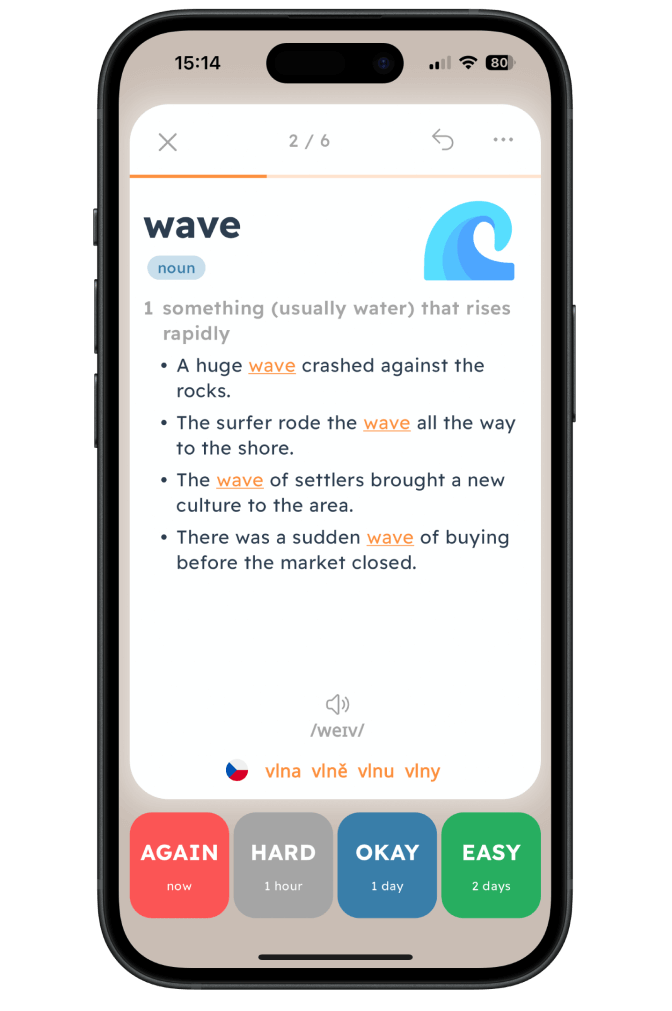
\includegraphics[width=0.6\textwidth]{src/figures/em-srs-flashcard.png}
    \caption{English Mind - SRS}
    \label{fig:em-srs-flashcard}
\end{figure}

\section{Application Workflow}

The application's learning process consists of two primary phases: vocabulary selection and practice. Figure \ref{fig:em-hta} illustrates the hierarchical breakdown of these tasks.

Users first browse the frequency-ordered vocabulary list, marking words as either "KNOWN" (already mastered) or "LEARNING" (to be studied). This initial classification ensures that learning efforts focus on appropriate vocabulary. Subsequently, words marked as "LEARNING" enter the practice phase, where they are studied through flashcards and systematically reviewed using spaced repetition.

\vspace{1cm}

\begin{figure}[!h]
    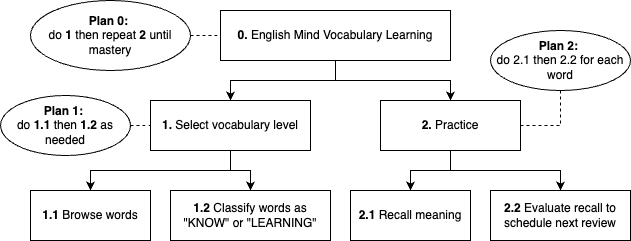
\includegraphics[width=1\textwidth]{src/figures/english_mind_workflow_THA.png}
    \caption{Hierarchical Task Analysis of English Mind's core learning workflow}
    \label{fig:em-hta}
\end{figure}
